\documentclass[a4paper,11pt, twocolumn]{article}
\usepackage[margin=0.8in]{geometry}
\usepackage{xcolor}
\usepackage{graphicx} %package to manage images
\graphicspath{ {./images/} }

\title{A2-02 AC Circuits And Passive Filters}
\author{Revision sheet}
\date{}

\usepackage{fancyhdr}
\pagestyle{fancy}
\fancyhead{} % clear all header fields
\renewcommand{\headrulewidth}{0pt} % no line in header area
\fancyfoot{} % clear all footer fields
\renewcommand{\footrulewidth}{0.4pt}
\fancyfoot[C]{\thepage} % page number in centre of the page
\fancyfoot[R]{\footnotesize Thomas Boxall \\ Images from WJEC E-Book} % right hand footer has author name on top line and images reference on bottom line
\fancyfoot[L]{\footnotesize A2-02 AC Circuits And Passive Filters \\ Revision sheet} % left hand footer has title of document on top line and 'Revision Sheet' on bottom line


\begin{document}

\maketitle
\thispagestyle{fancy}

% CONTENTS OF THE REVISION SHEET HERE
\section{Waves}
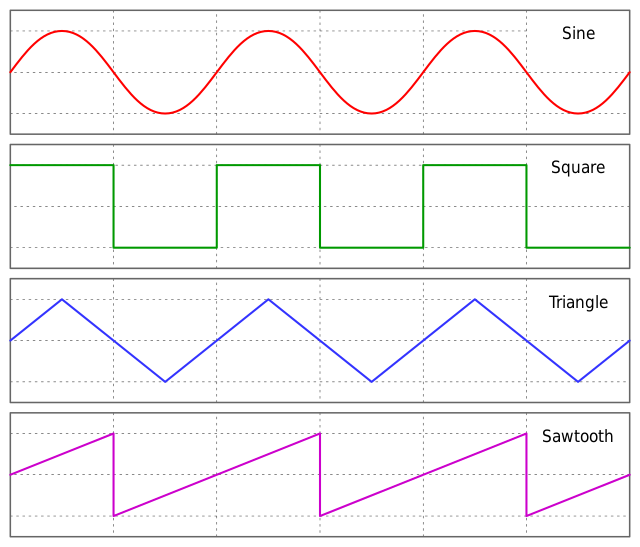
\includegraphics[width=0.45\textwidth]{basicWaveforms.png}\\
Each of the waves above have the same frequency and amplitude but each would produce a different sound or tone. 

\section{Frequencies}
A sine wave only contains one frequency. Other waves contain multiple frequencies - the fundamental frequency (this is the note that we recognise) and a series of higher, weaker frequencies (called harmonics). 
\subsection{Fourier Analysis}
Any waveform can be made form a series of sine waves of different amplitudes and frequencies - the waves form a 'fourier series'. A square wave is formed from an infinite series of odd harmonics of decreasing amplitude.
\subsection{Stages of Fourier Analysis}
This starts off with just the fundamental.\\
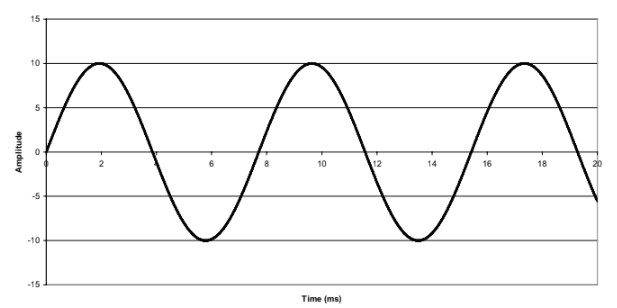
\includegraphics[width=0.45\textwidth]{fourier1.jpg}\\
Then you add more harmonics.\\
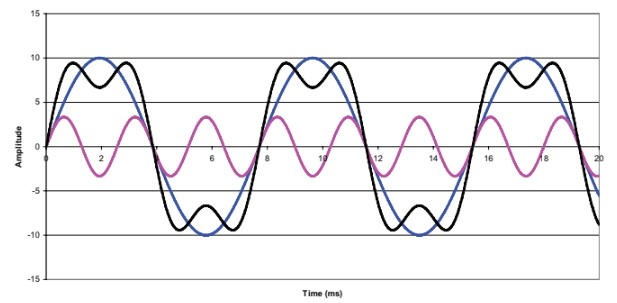
\includegraphics[width=0.45\textwidth]{fourier2.jpg}\\
As you add more and more harmonics gives a result which is looking more square like.\\
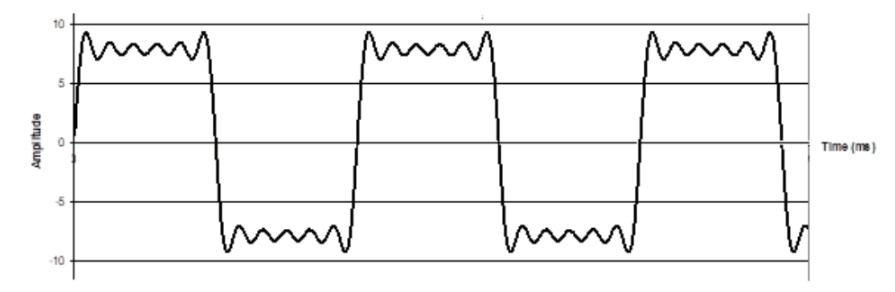
\includegraphics[width=0.45\textwidth]{fourier3.jpg}\\
Fourier's theorem states that to create the perfect square requires an infinite number of odd harmonics. 
\subsection{Frequency Spectrum Analysis}
Frequencies can be represented as both their waveform and on a frequency spectrum. Shown below is the waveform and frequency spectrum for a 1KHz sine wave.\\
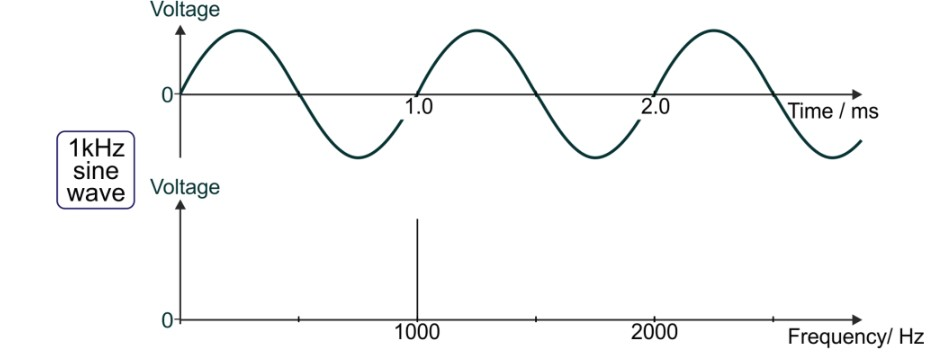
\includegraphics[width=0.45\textwidth]{sineFrequencySpectrum.jpg}\\
Square waves can also be represented in the same way. There are more frequencies required to represent a square wave on a frequency spectrum due to the nature of the composition of a square wave.
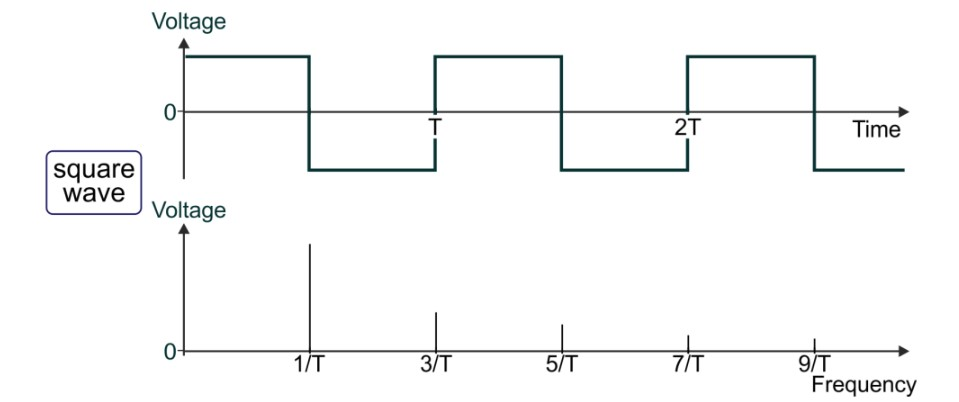
\includegraphics[width=0.45\textwidth]{squareFrequencySpectrum.jpg}

\section{Bandwidth}
Bandwidth is the \textit{range of frequencies required to make up the signal}. The bandwidth for a sine wave is zero whereas for a square wave, it is infinite. \\
$Bandwidth = f_{max} - f_{min}$\\
\subsection{Bandwidth Limiting}
In real world situations, bandwidth has to be limited as humans can hear between 20Hz and 20KHz, it would be completely impractical to transmit this down the phone lines for example.
\subsubsection{Telephone}
Bandwidth is limited to 300Kz to 3.1KHz. This gives a bandwidth of 3.1KHz. \\
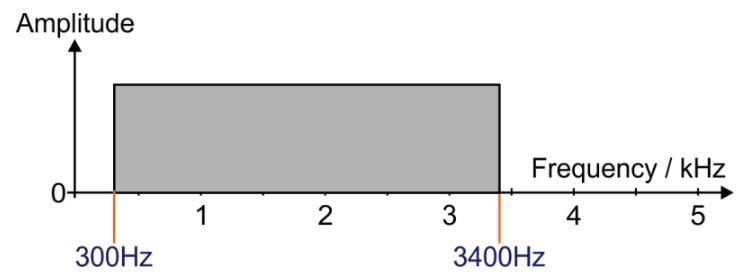
\includegraphics[width=0.45\textwidth]{telephoneBandwidth.jpg}\\
Bandwidth is represented on graphs like the one above - as a rectangle. 
\subsubsection{FM Radio}
FM Radio's bandwidth is limited to 30Hz to 15KHz.

\section{Filters}
Filter circuits are used to control the bandwidth allocated to speech and music signals in communication systems. The filters shown here are passive filters, there are also active filters (covered in the Audio Systems unit).
\subsection{Break Frequency}
This is the value at which the filter makes a change. For a low pass filter, everything below the filter passes but everything above is cut off. \\
$\displaystyle f_{b}=\frac{1}{2 \pi R C}$
\subsection{Impedance}
Resistance and Reactance are types of impedance. \\
$\displaystyle Z = \sqrt{R^2 + X_c\ ^2}$
\subsubsection{Frequency Response Curves}
This is the graph of the output of the filter based off of different frequency inputs. It is plotted on log-log axis.
\subsection{Reactance}
In AC circuits, capacitors behave differently to in DC Circuits. They have a measure of the opposition of the capacitor to an AC current - the capacitive reactance ($X_C$), measured in Ohms.\\
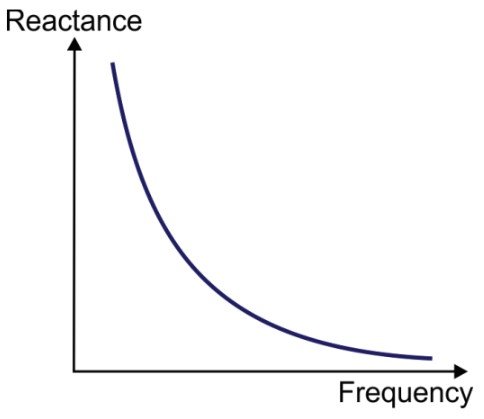
\includegraphics[width=0.45\textwidth]{reactance.jpg}\\
$\displaystyle X_C = \frac{1}{2 \pi f C}$
\subsection{Inductors}
This is a coil of wire which, when a voltage is applied, generates a magnetic field. As the field grows, it generates a current in the coil in the opposite direction (Back EMF). This reduces current flow. Once the field stops growing, there is no more back EMF therefore no opposition to current behaves like a short circuit).\\
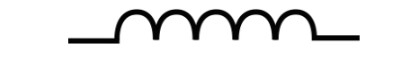
\includegraphics[width=0.45\textwidth]{inductor.jpg}\\
Inductance is measured in Henries (H). Inductance has the letter L in equations.
\subsubsection{Inductive Reactance}
Inductive reactance ($X_L$) is the opposition to the flow of an AC current.\\
$\displaystyle X_L = 2 \pi f L$ 
\subsection{Different Types of Filters}
\subsubsection{Low-Pass Filter}
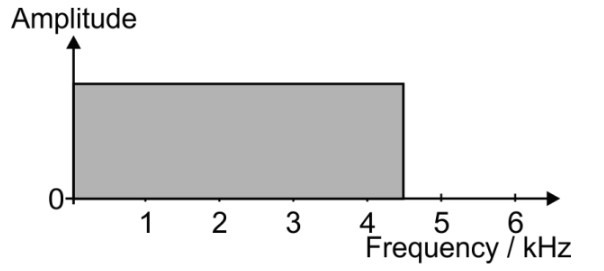
\includegraphics[width=0.45\textwidth]{lpfBasicGraph.jpg}\\
Shown above is the output we want from a low-pass filter.\\
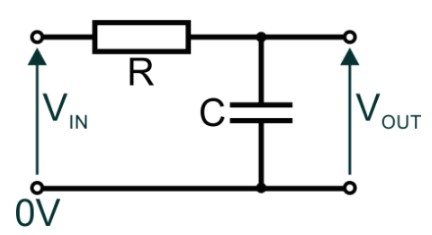
\includegraphics[width=0.45\textwidth]{lpfCircuit.jpg}\\
Shown above is the circuit diagram for the low-pass filter.\\
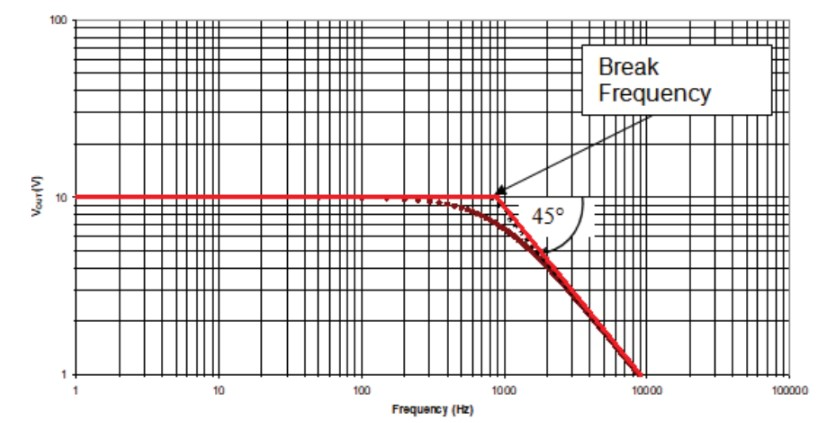
\includegraphics[width=0.45\textwidth]{lpfFreqResp.jpg}\\
Shown above is the frequency response curve for the low-pass filter.\\
$\displaystyle Gain = \frac{X_c}{\sqrt{X_c\ ^2 + R^2}}$\\
$\displaystyle V_{out} = V_{in} \times \frac{X_c}{\sqrt{X_c\ ^2 + R^2}}$
\subsubsection{High-Pass Filter}
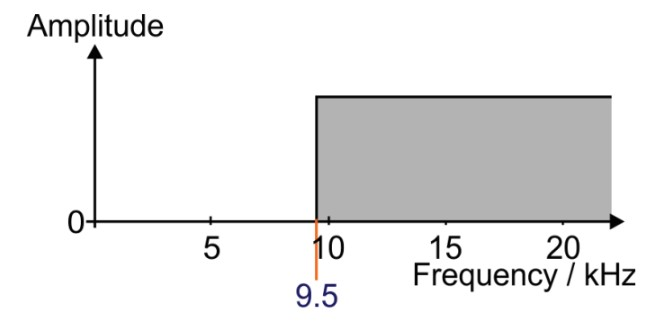
\includegraphics[width=0.45\textwidth]{hpfBasicGraph.jpg}\\
Shown above is the output we want form a high-pass filter.
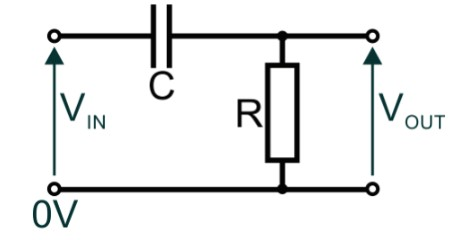
\includegraphics[width=0.45\textwidth]{hpfCircuit.jpg}\\
Shown above is the circuit diagram for the high-pass filter.\\
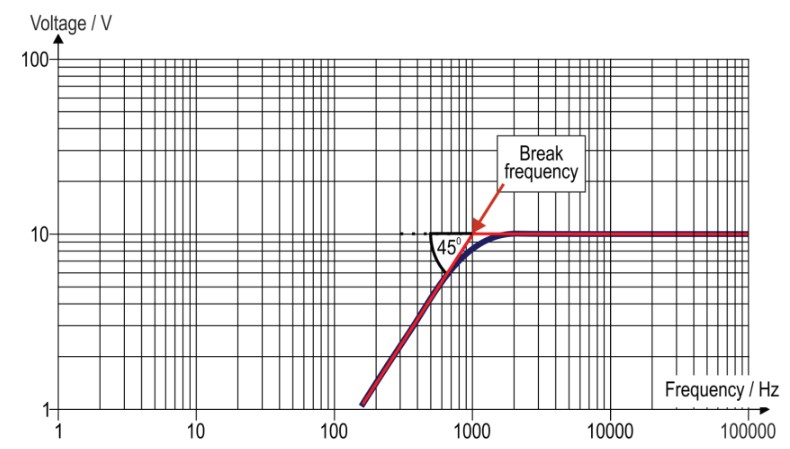
\includegraphics[width=0.45\textwidth]{hpfFreqResp.jpg} \\
Shown above is the frequency response curve for the high-pass filter.\\
$\displaystyle Gain = \frac{R}{\sqrt{X_c\ ^2 + R^2}}$\\
$\displaystyle V_{out} = V_{in} \times \frac{R}{\sqrt{X_c\ ^2 + R^2}}$
\subsubsection{Band-Pass Filter}
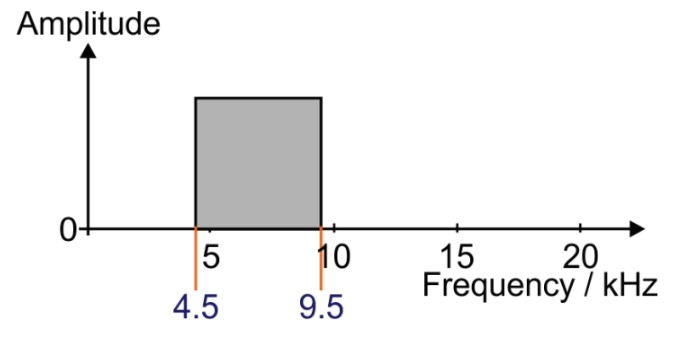
\includegraphics[width=0.45\textwidth]{bpfBasicGraph.jpg}\\
Shown above is the output we want from a band-pass filter.\\
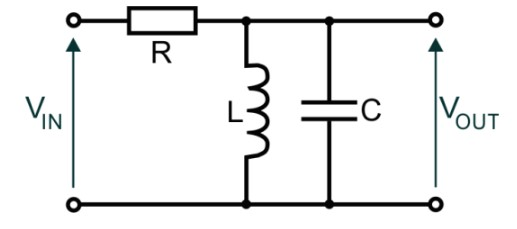
\includegraphics[width=0.45\textwidth]{bpfCircuit.jpg}\\
Shown above is the circuit diagram for the band-pass filter.\\
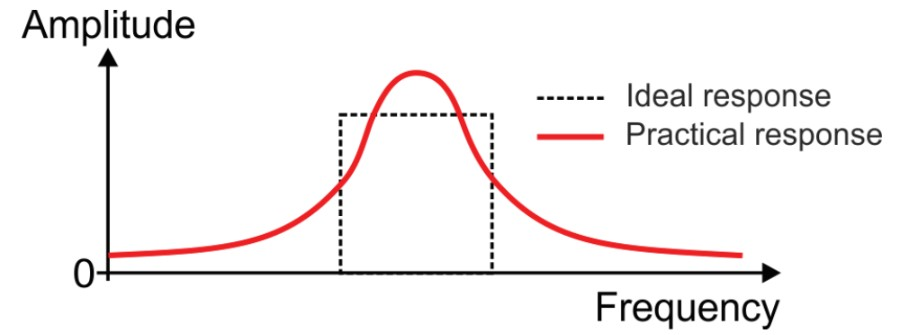
\includegraphics[width=0.45\textwidth]{bpfFreqResp.jpg}\\
Shown above is the frequency response curve for the band-pass filter. A poor response would result in a similar shape with lower amplitude. \\
At the resonate frequency ($f_o$), $V_{out}$ is at its maximum value (the peak on the frequency response curve). \\
$\displaystyle f_o = \frac{1}{2 \pi \sqrt{LC}}$\\
\textbf{Dynamic resistance} is the effective resistance of the parallel inductor, capacity combination at resonance.\\
$\displaystyle R_D = \frac{L}{r_L C}$\\
\textbf{Bandwidth} of a bpf is the range of frequencies for which $V_{out}$ is above $\frac{1}{\sqrt{2}}$ (70\%) of its maximum. \\
\textbf{Q-Factor} measures how good the filer is and how tight the frequency response is. A high q-factor is better and it has a taller peak on the graph. A low q-factor is worse and it has a stumpier peak on the graph. \\
$\displaystyle Q-Factor = \frac{f_o}{bandwidth} = \frac{2 \pi f_o L}{r_L}$

\subsection{Loading}
When a load is added to a filter, it is in parallel with a component. This changes the frequency response. The solution to this is to add a unity gain buffer to the output of the filter (shown below for a hpf). The op-amp has a very high input impedance therefore it doesn't load the filter, this doesn't affect the frequency response. This is the same method used for all three types of filters.\\
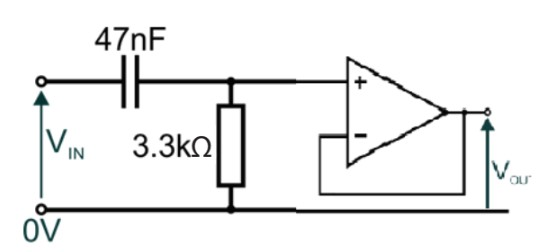
\includegraphics[width=0.45\textwidth]{load.jpg}




\end{document}
